\documentclass{standalone}
\usepackage{tikz}
\usetikzlibrary{calc, shapes, patterns}

\begin{document}
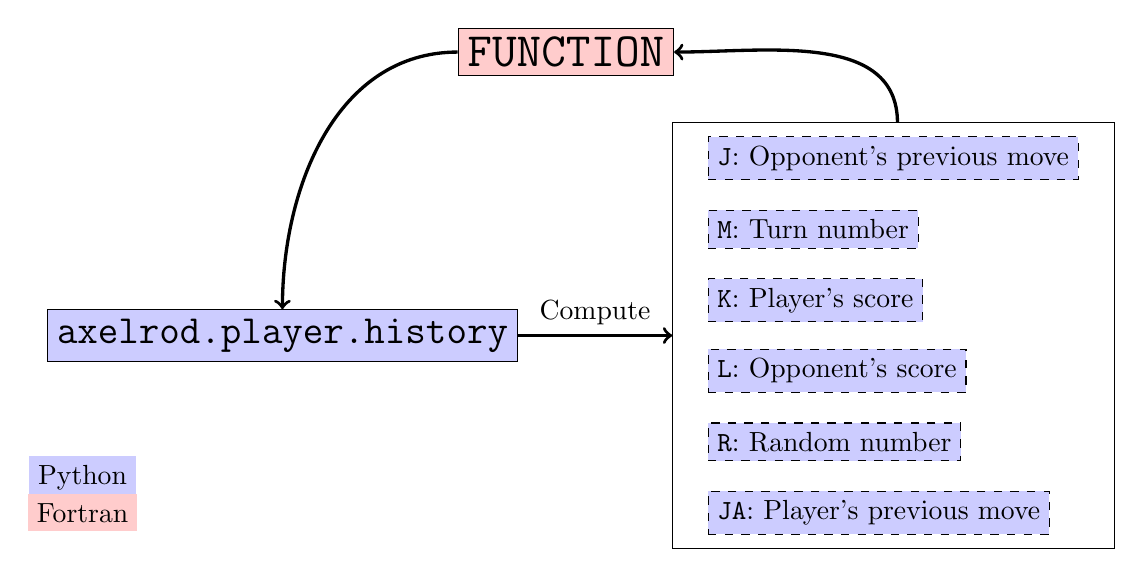
\begin{tikzpicture}[scale=.9]
    \node (axelrod_player) at (0, 0) 
        [draw, fill=blue!20, right] 
        {\Large \texttt{axelrod.player.history}};

    \node (fortran_function) at ($(axelrod_player) + (4, 4)$) 
        [draw, fill=red!20] 
        {\LARGE \texttt{FUNCTION}};

    % Computations
    \node (opp_previous_move) at ($(axelrod_player) + (6, 2.5)$) 
        [draw, fill=blue!20, dashed, right] 
        { \texttt{J}: Opponent's previous move};
    \node (current_move_number) at ($(axelrod_player) + (6, 1.5)$) 
        [draw, fill=blue!20, dashed, right] 
        { \texttt{M}: Turn number};
    \node (player_score) at ($(axelrod_player) + (6, .5)$) 
        [draw, fill=blue!20, dashed, right] 
        { \texttt{K}: Player's score};
    \node (opponent_score) at ($(axelrod_player) + (6, -.5)$) 
        [draw, fill=blue!20, dashed, right] 
        { \texttt{L}: Opponent's score};
    \node (random_number) at ($(axelrod_player) + (6, -1.5)$) 
        [draw, fill=blue!20, dashed, right] 
        { \texttt{R}: Random number};
    \node (player_previous_move) at ($(axelrod_player) + (6, -2.5)$) 
        [draw, fill=blue!20, dashed, right] 
        { \texttt{JA}: Player's previous move};


    \draw ($(opp_previous_move.east) + (.5, .5)$) 
                rectangle 
          ($(player_previous_move.west) + (-.5, -.5)$);

      \draw [very thick, ->] 
          (axelrod_player.east) -- node [above] {Compute} 
          ($(axelrod_player) + (5.5, 0)$);

      \draw (12, 3) edge[out=90, in=0, ->, very thick] 
          (fortran_function);
      \draw (fortran_function) edge[out=180, in=90, ->, very thick] 
          (axelrod_player);

    \node at (.5, -2) [fill=blue!20] {Python};
    \node at (.5, -2.5) [fill=red!20] {Fortran};
\end{tikzpicture}
\end{document}
